\documentclass[a4paper]{article}

\usepackage[french]{babel}
\usepackage[utf8]{inputenc}
\usepackage{graphicx}
\usepackage{pdfpages}

\title{Small World : Rapport de Modélisation \\ INSA de Rennes - 4INFO}

\author{Axel CARO, Maximilien RICHER}

\date{\today}

\begin{document}
\maketitle

\paragraph{}
Ce document présente les résultats de la phase de modélisation du projet de quatrième année proposé en enseignement de \textit{Programmation et Modélisation orientées objet}.

\newpage

\section*{Introduction}
\paragraph{}
Le projet proposé consiste en la réalisation d'un jeu vidéo tour par tour, basé sur le jeu de plateau \textit{SmallWorld}. Au cours d'une partie, les joueurs s'affrontent pendant un certain nombre de tours, afin prendre le contrôle d'un territoire. Ce projet met l'accent sur les différentes phases de la réalisation d'un projet d'application orientée objet. La modélisation, l'utilisation de patrons de conceptions, l'organisation du code, l'implémentation, l'utilisation de librairies dynamiques, l'interfaçage entre plusieurs langages, la gestion d'IHM et les phases de tests sont des points clés des objectifs pédagogiques de ce projet.

\section{Présentation des règles du jeu}

\subsection{But du jeu}
\paragraph{}
Le but de SmallWorld est d'accumuler des points.
À la fin de chaque tour de jeu, le joueur compte les points gagnés et les ajoutes à son total. Au bout d'un nombre de tour défini au préalable, le jeu s'arrête et le joueur ayant le plus de point remporte la partie. Une partie peut également s'interrompre si un des joueurs élimine l'ensemble des unités de l'adversaire. Un joueur qui ne possède plus d'unités perd la partie, quel que soit son total de point.

\subsubsection{Plateau de jeu}
\paragraph{}
Le jeu se déroule sur une plateau quadrillé de cases carré dont la dimension dépend du nombre de joueurs et de la durée de la partie.\label{map_gen} Il est composé de cases de différents types : plaine, mer, montagne et forêt.La carte est généré de manière aléatoire, mais doit contenir le même nombre de case de chaque type.

\subsubsection{Unité}
\paragraph{}
Des unitées sont placées sur le plateau, sur lequel elles peuvent se déplacer.

\subsubsection{Races et comptage des points en fin de tour}

\paragraph{}
\textbf{Configurations conseillées}
\begin{itemize}
    \item 2 joueurs, plateau de 6 par 6, 5 tours de jeu : 4 unités par joueur
    \item 2 joueurs, plateau de 10 par 10, 20 tours de jeu : 6 unités par joueur
    \item 2 joueurs, plateau de 14 par 14, 30 tours de jeu : 8 unités par joueur
\end{itemize}

\subsubsection{Préparation}
\paragraph{}
La préparation du jeu necéssite que le joueur choississe le type de partie parmis les configurations proposées, 

\subsection{Déroulement d'un tour de jeu}
\paragraph{}
Chaque \em{tour de jeu} est constitué de plusieurs \em{tours de joueurs}. Ces tours sont séquentiels. Lors du premier tour de jeu, le joueur jouant le premier tout est tiré au hasard, et cet ordre est conservé durant le reste de la partie.
\paragraph{}
\textbf{Déroulement du tour}
\begin{itemize}
    \item Début du tour
    \item Déplacement des unités et combats
    \item Décompte des points
    \item Fin du tour
\end{itemize}

\subsection{Déplacement et combat}


\section{Modélisation UML}
\paragraph{}
La phase de modélisation nous a conduit à réaliser plusieurs diagrammes UML, afin de représenter différents aspects de notre application. Nous présentons ci-après ces diagrammes, en explicitant leur contenu.

\subsection{Diagramme de paquetage}
\paragraph{}
Le diagramme suivant illustre la structuration à gros grain du code de notre application. On y retrouve les classes et interfaces que nous détaillerons dans la section \ref{DDC}. Ce diagramme illustre les interactions entre les regroupements de classes. On ne parle pas ici de \textit{package} proprement dit, car le choix du \textbf{C\#} comme langage de programmation ne permet pas l'utilisation de paquetages. Il s'agit d'un découpage ayant pour but de présenter la structure des différentes parties de l'application, sans détailler les interactions internes à chaque regroupement.

\paragraph{}
On distingue 7 regroupements, en plus de l'application principale (\textit{SmallWorld}) :
\begin{enumerate}
\item \textit{Tile} : gestion des cases du terrain de jeu.
\item \textit{Map} : gestion du terrain de jeu.
\item \textit{Race} : gestion des différentes races jouables.
\item \textit{Unit} : gestion des unités.
\item \textit{Player} : gestion des joueurs.
\item \textit{Game} : gestion de la partie.
\item \textit{SaveLoad} : gestion de la sauvegarde et du chargement de parties.
\end{enumerate}

\paragraph{}
Les interactions entre ces différents regroupements sont symbolisées par les flèches présentes sur le diagramme. Par exemple, le groupement \textit{Map} utilise des membres du groupement \textit{Tile}. Les interactions ainsi mises en valeur présentent bien la mise en cascade des regroupements, selon les données modélisées.

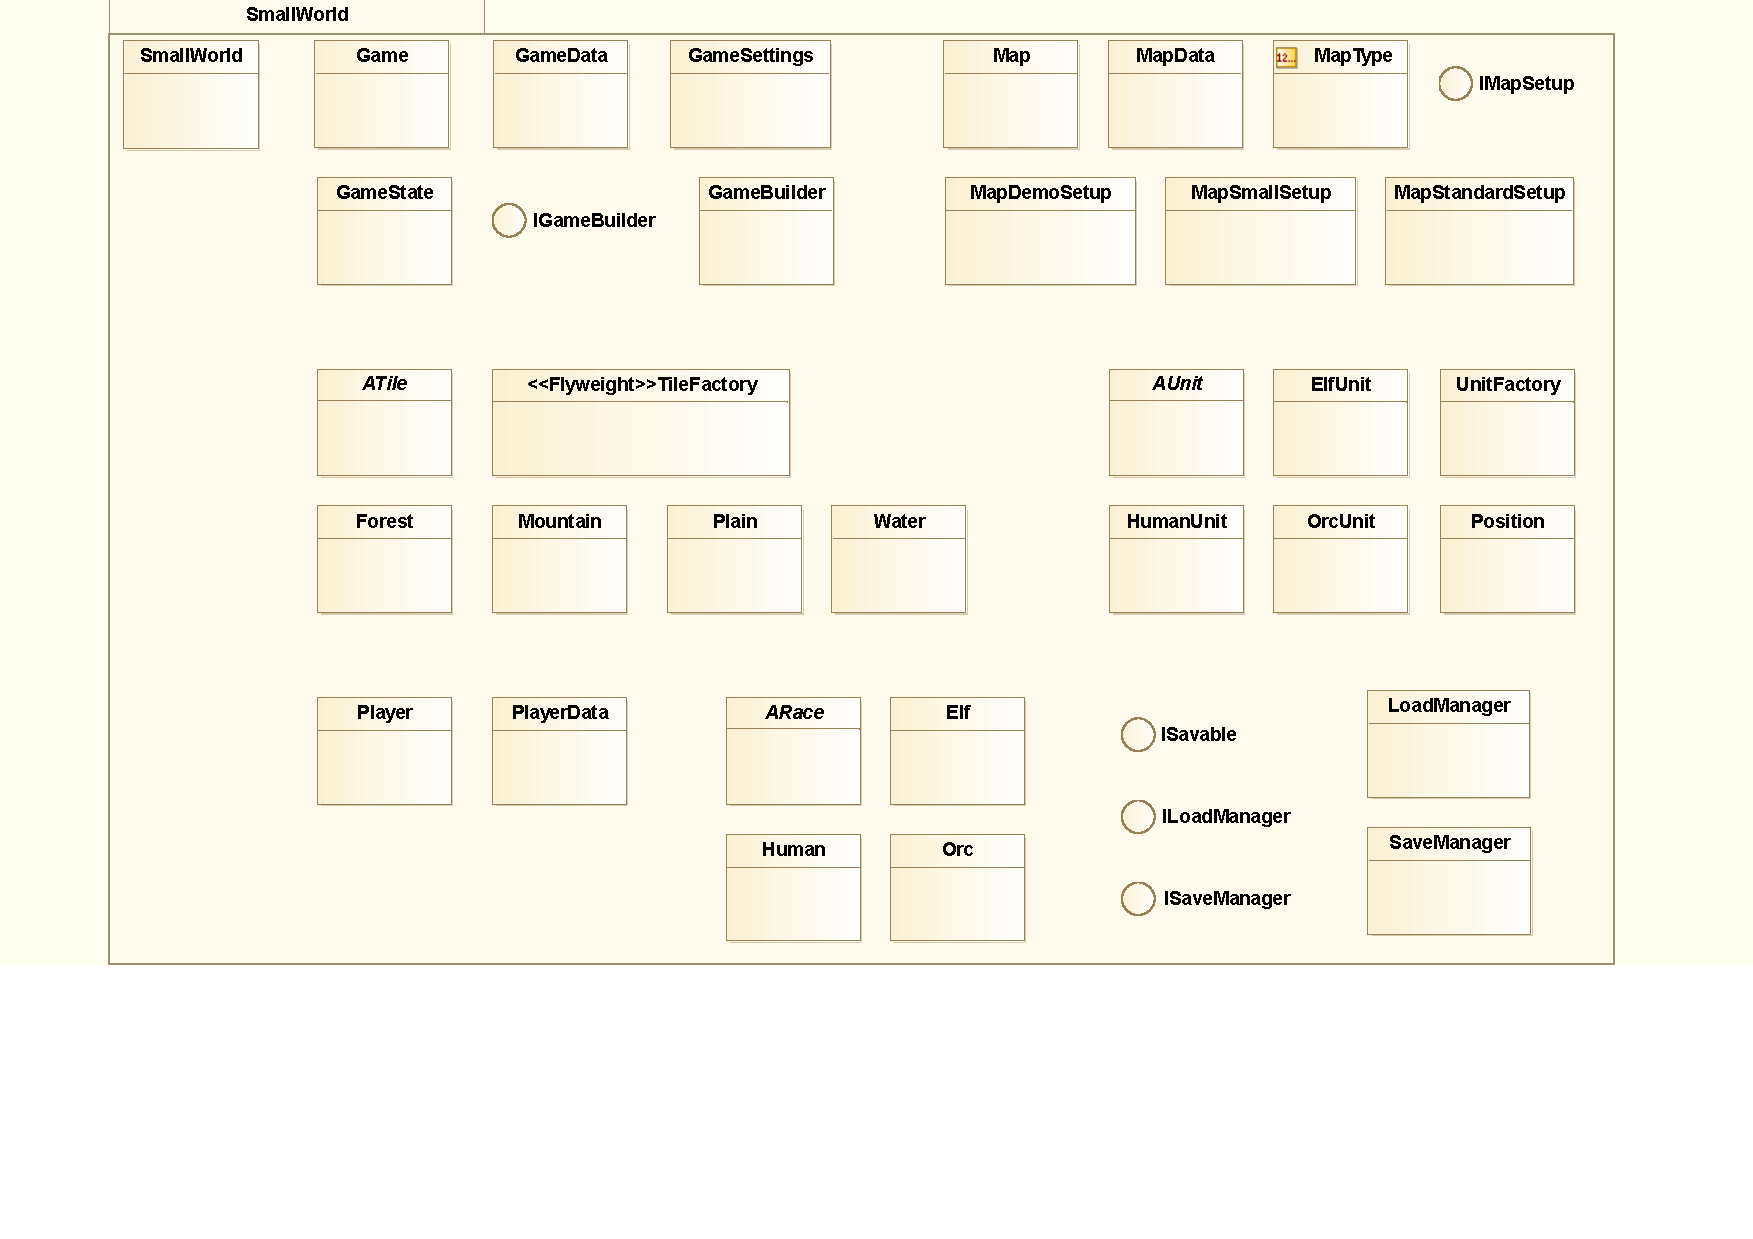
\includepdf[landscape=true]{images/packageDiagram.pdf}

\subsection{Diagramme de classes}
\label{DDC}
\paragraph{}
Le diagramme suivant illustre l'organisation en classes de notre application.

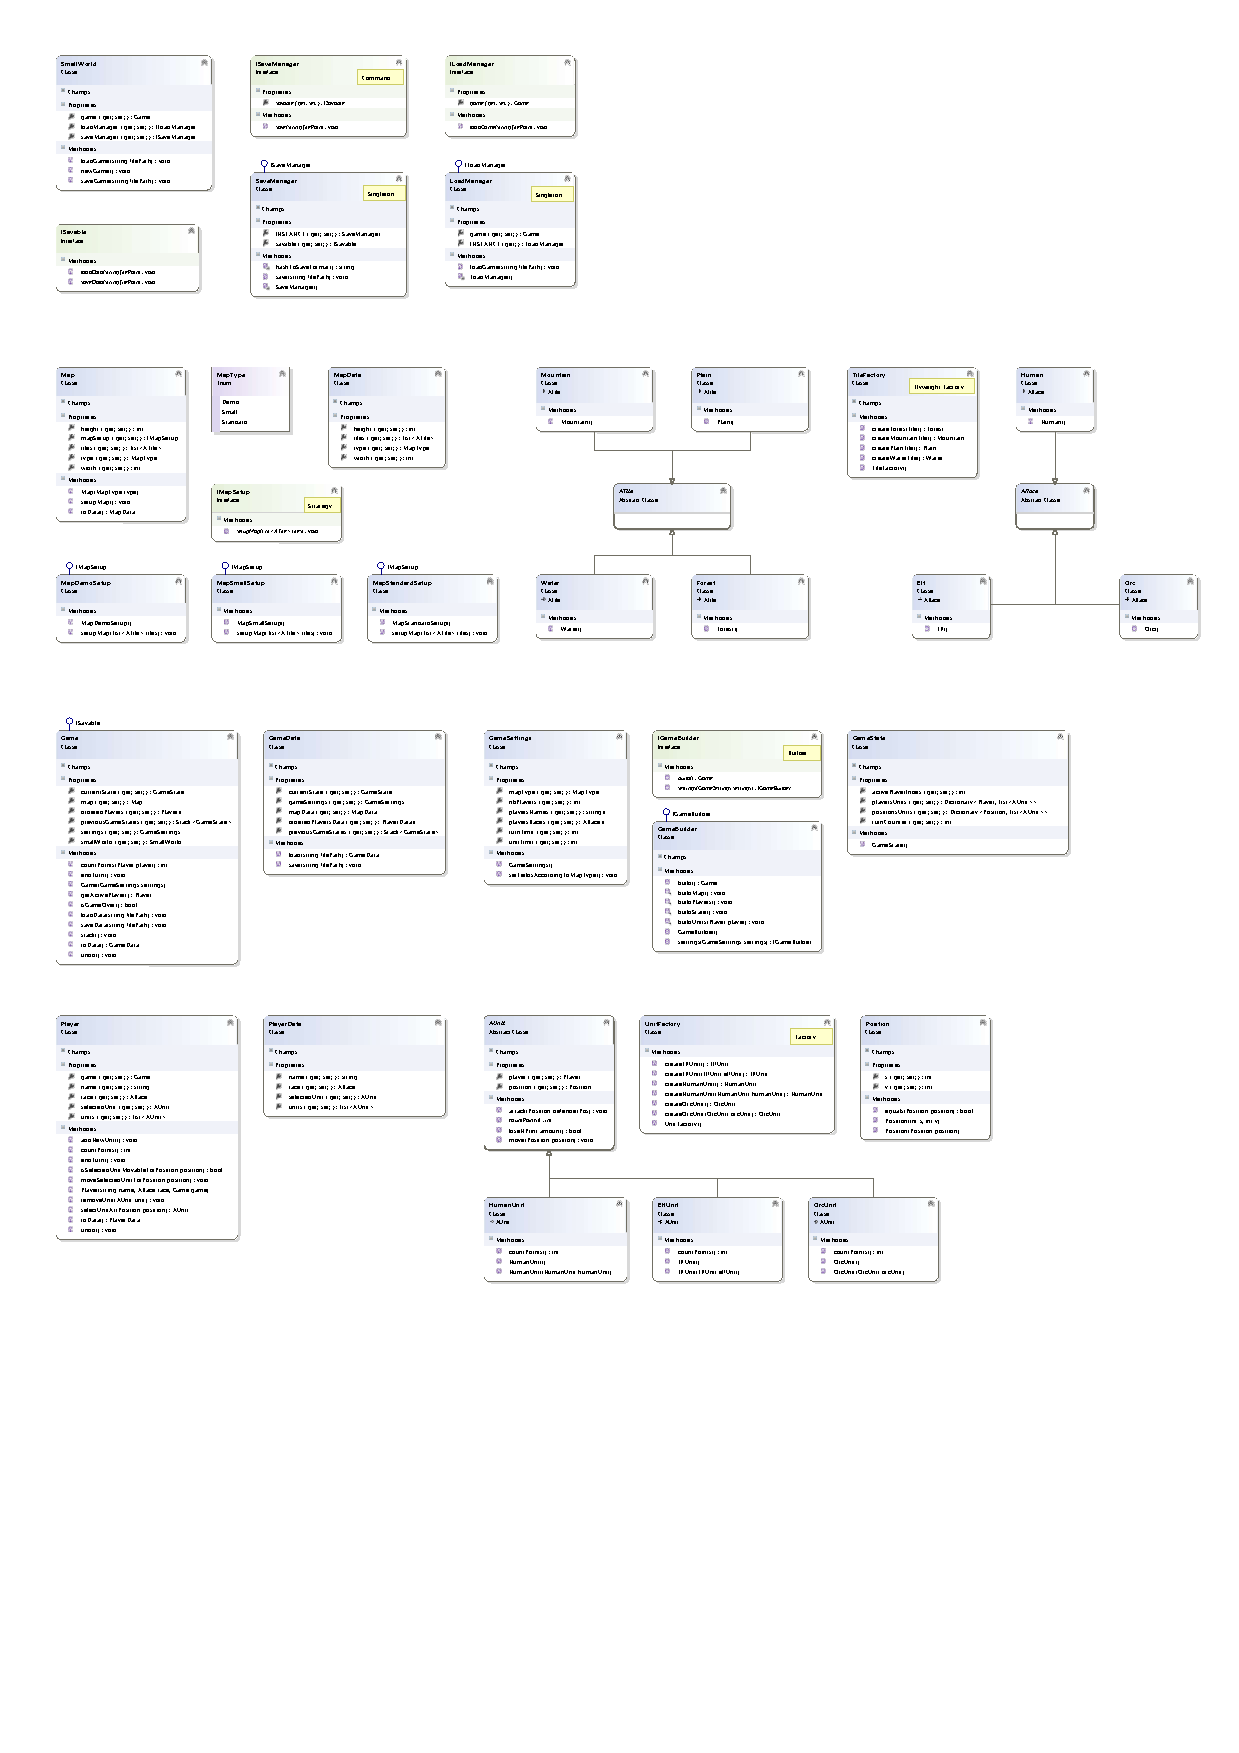
\includepdf{images/classDiagram.pdf}

\subsection{Diagrammes d'interaction}

\subsubsection{Diagramme de séquence : initialisation d'une partie}

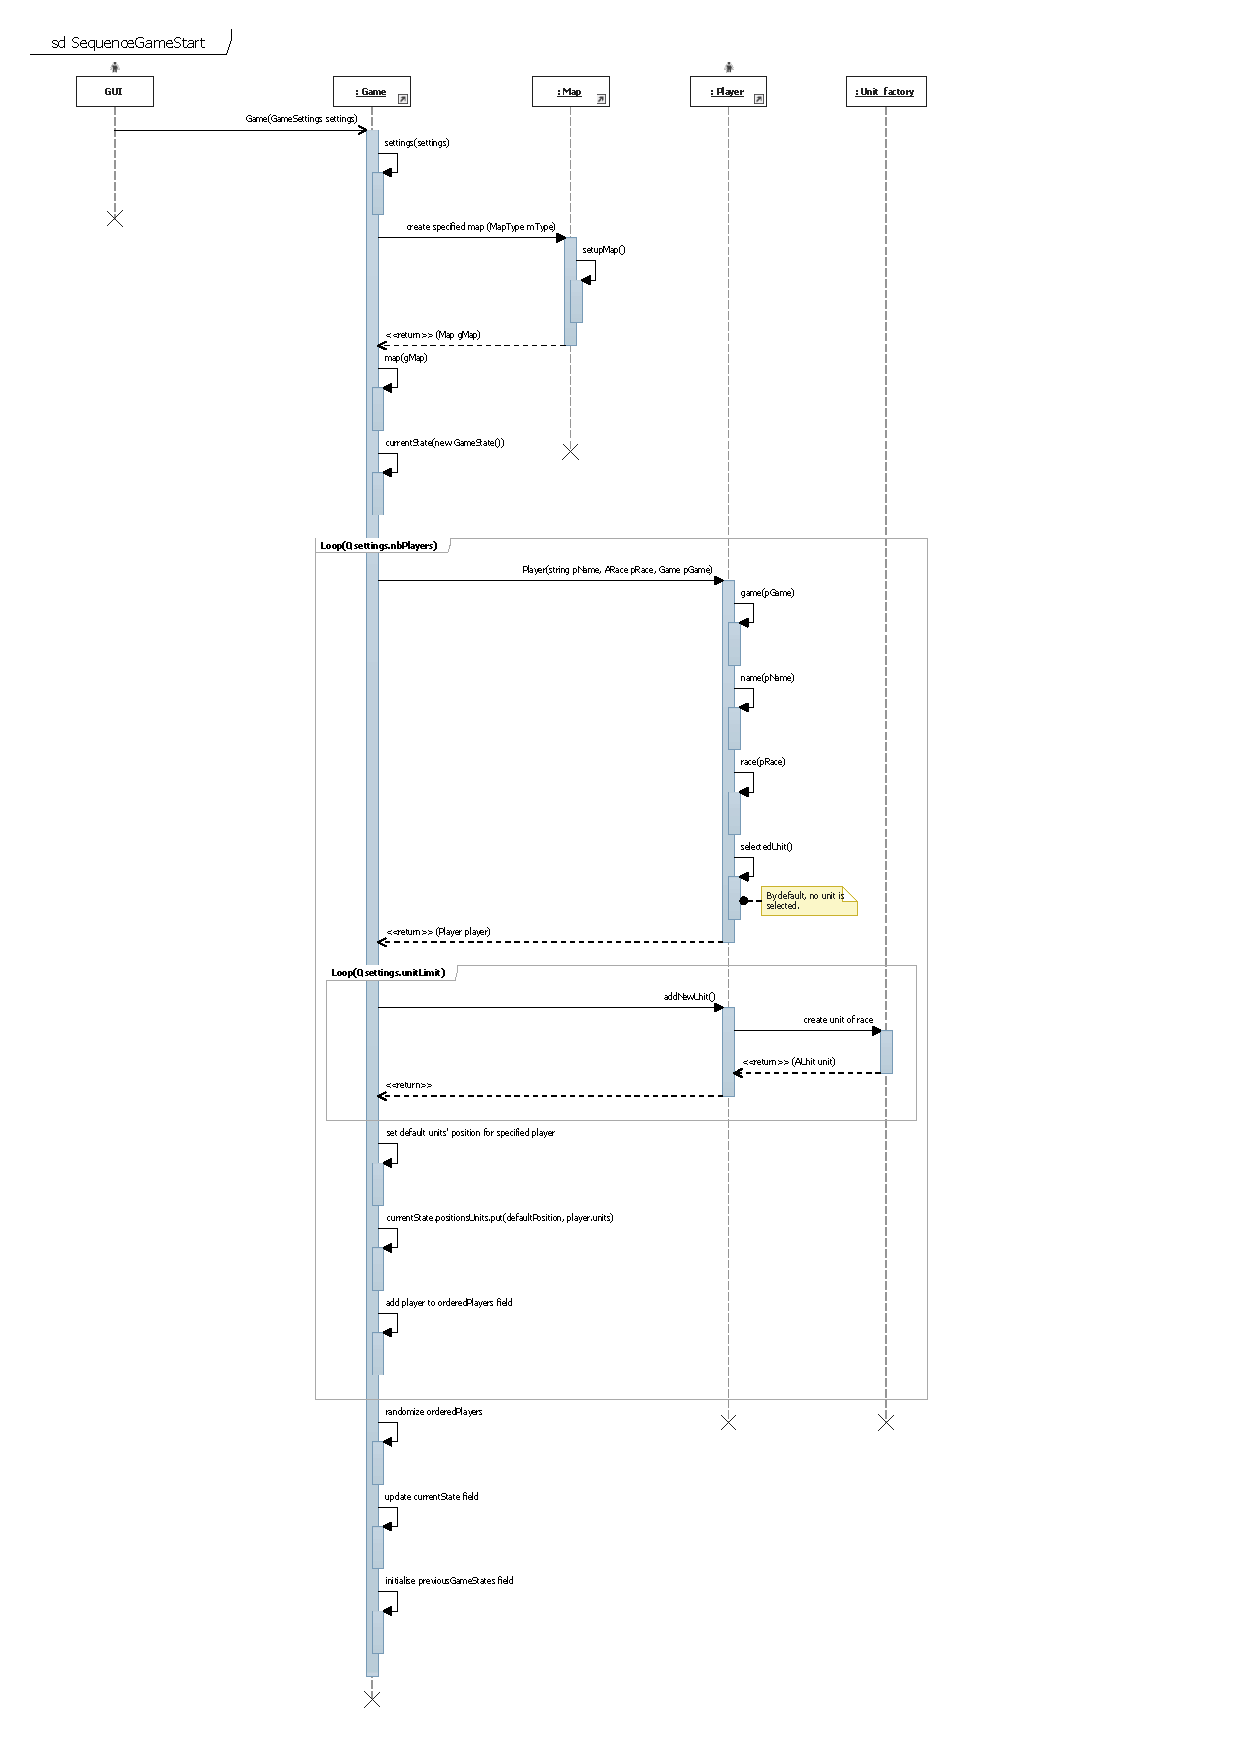
\includepdf{images/gameInitialisationSequenceDiagram.pdf}

\subsubsection{Diagramme de séquence : déroulement d'un tour}

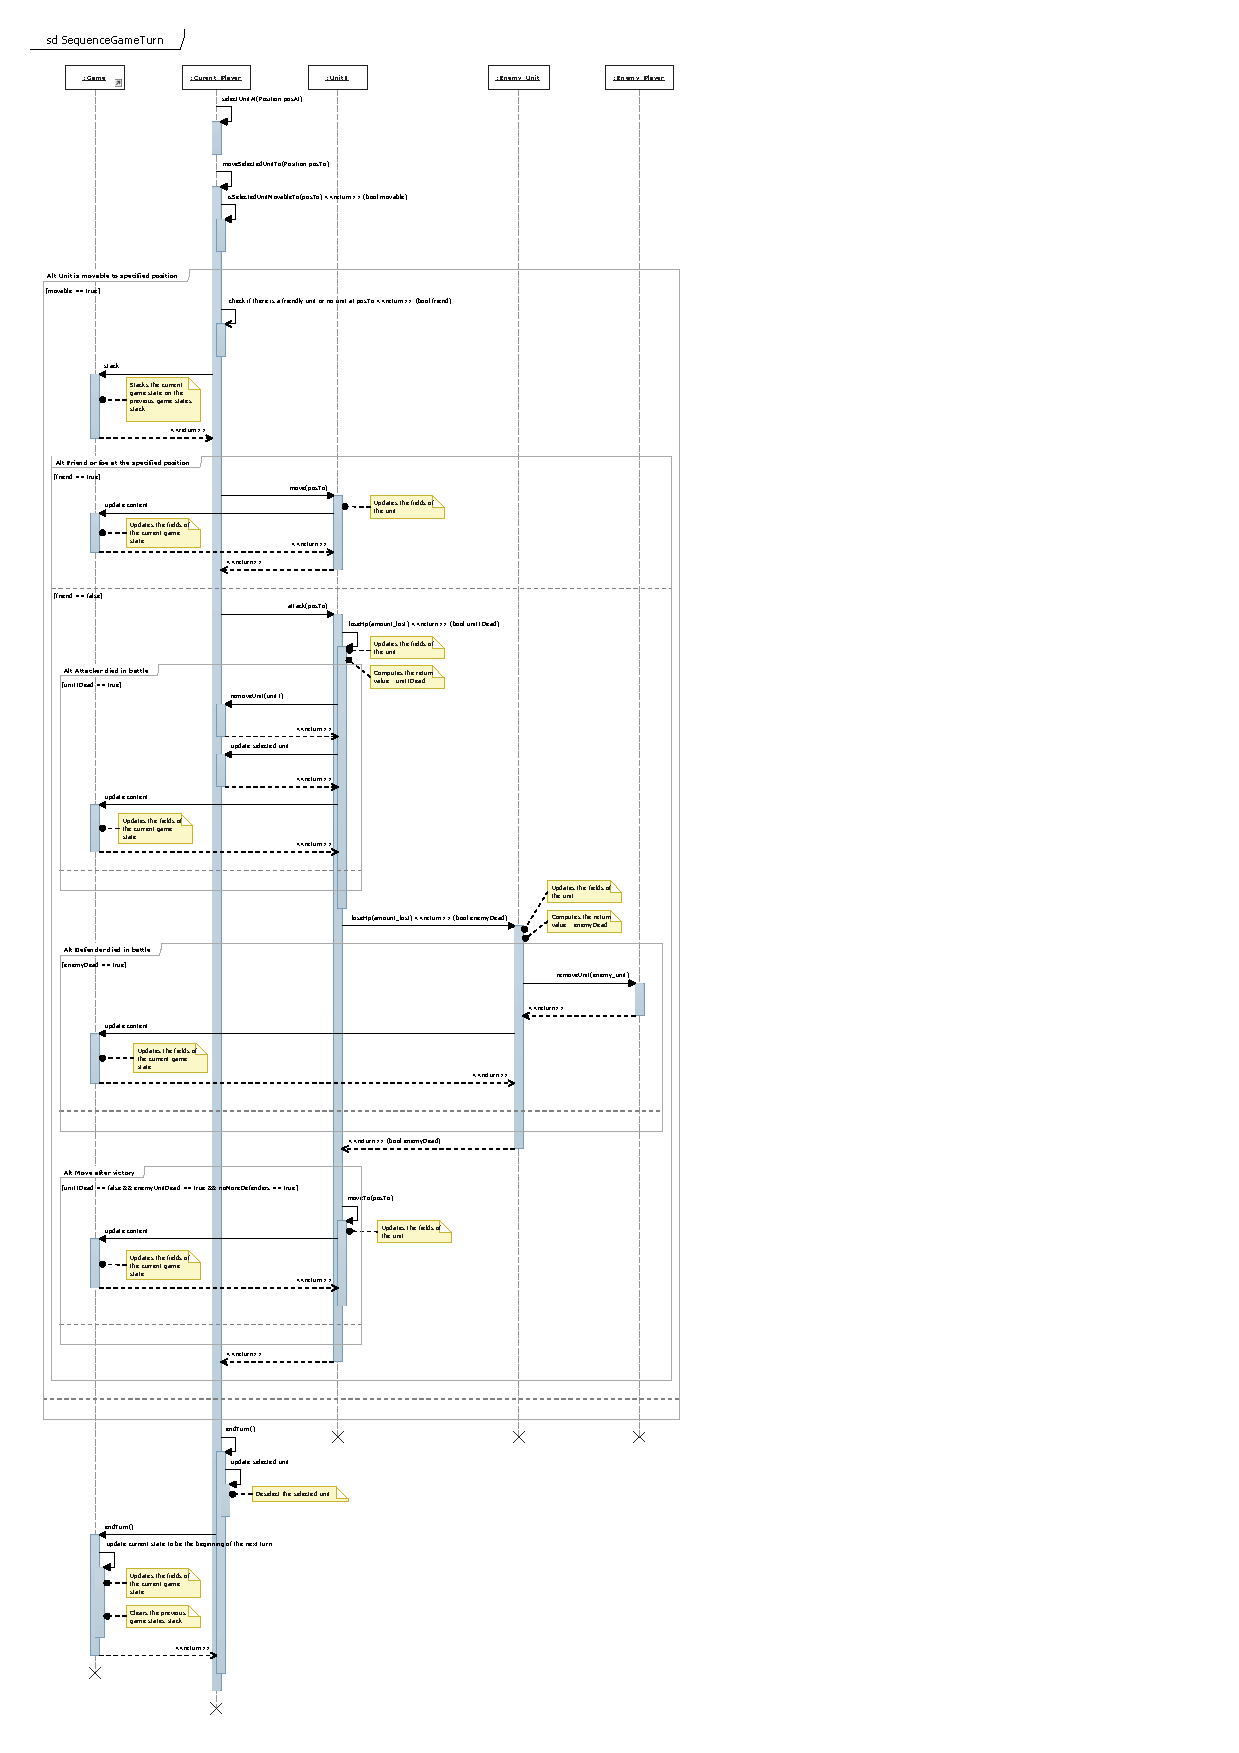
\includepdf{images/gameTurnSequenceDiagram.pdf}

\subsection{Diagramme d'états-transitions : gestion d'une unité}

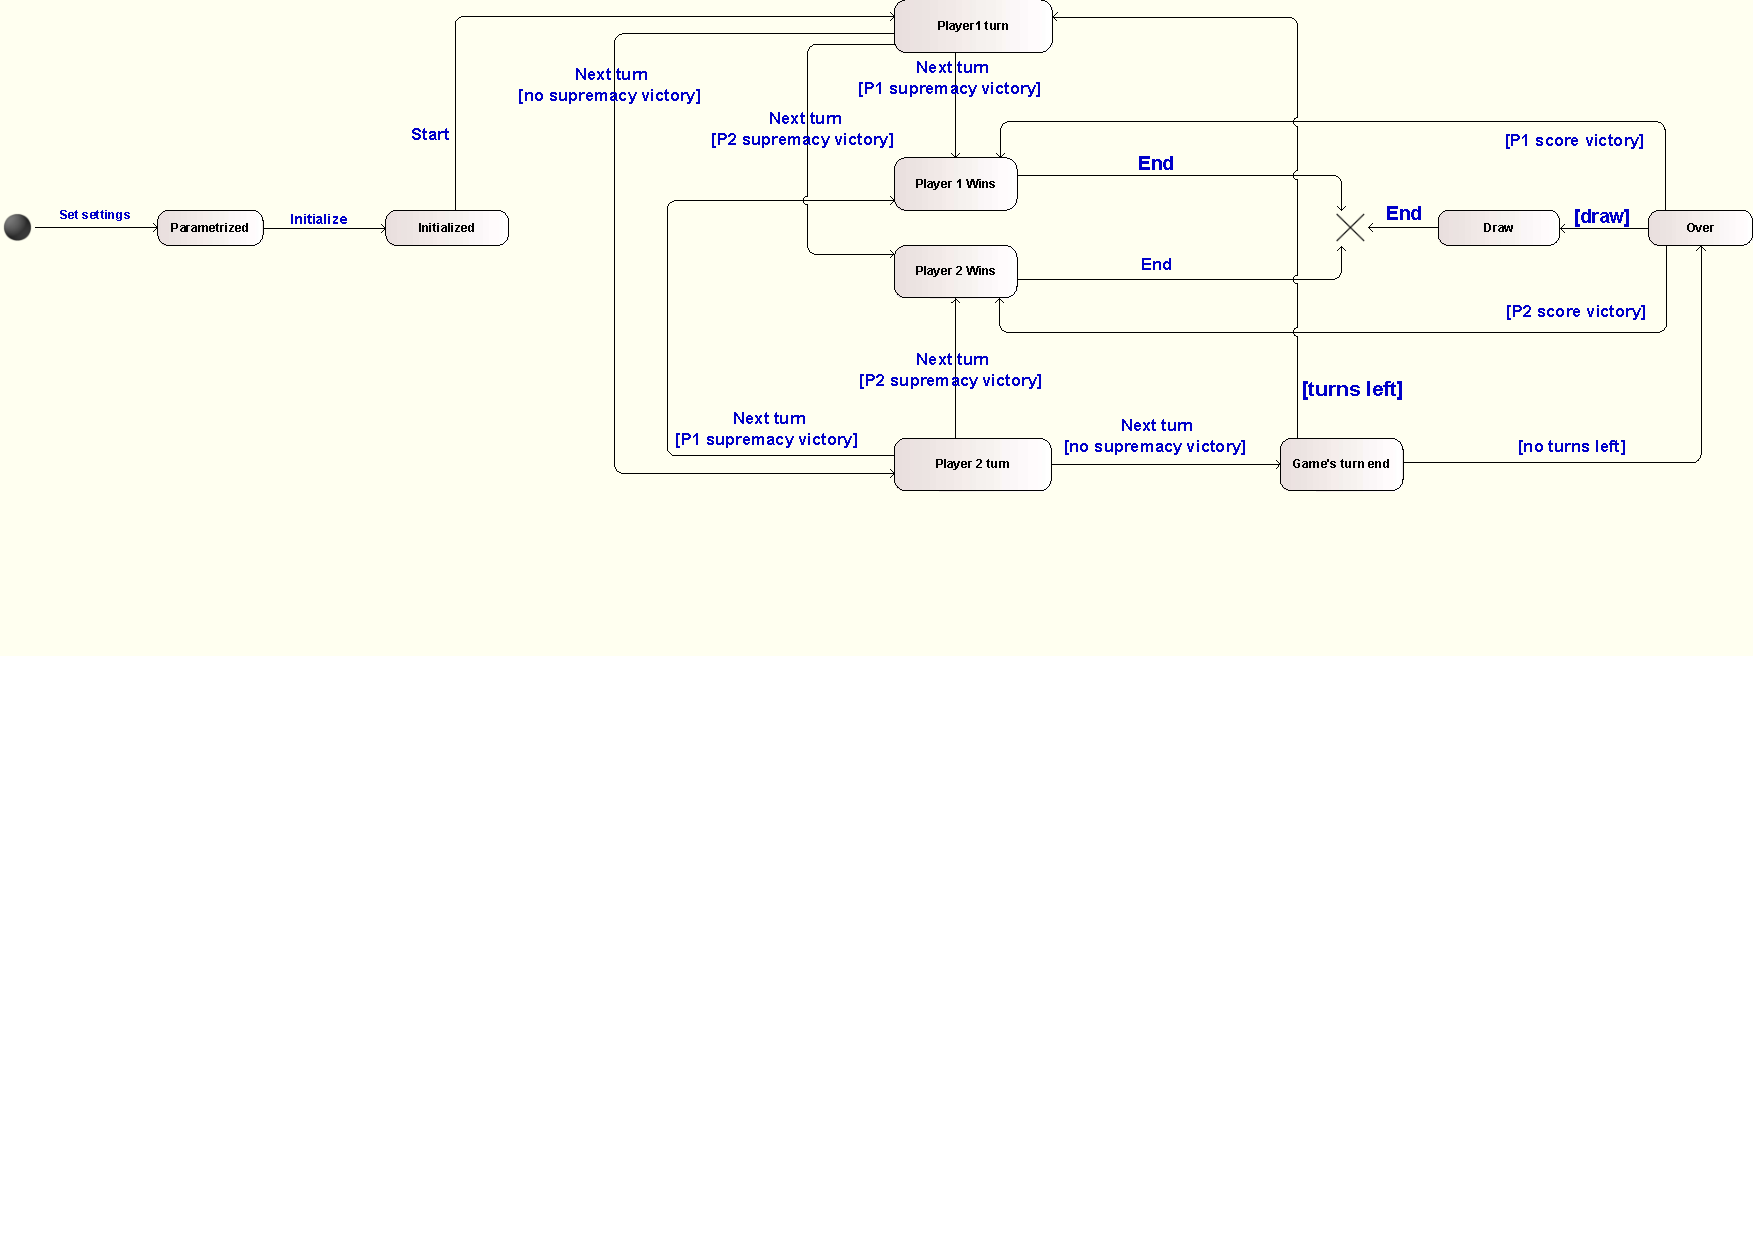
\includepdf{images/gameStatechart.pdf}

\end{document}
